\documentclass[a4paper,10pt]{report}

\usepackage[utf8]{inputenc}
\usepackage[frenchb]{babel}
\usepackage[T1]{fontenc}
\usepackage[top=2cm, bottom=2cm, left=2cm, right=2cm]{geometry}
\usepackage{listings}
\usepackage{hyperref}
\usepackage{color}
\usepackage{fancyhdr}
\usepackage{graphicx}
\usepackage{dirtree}

\title{Rapport Technique}

\pagestyle{fancy}
\fancyhead[L]{coucou}

\author{Florian Barrois \and Nicolas Devillers \and Valentin Jeanroy \and Mehdi Loisel \and Jean Mercadier \and Ismail Taleb \and Willeme Verdeaux}

\definecolor{dkgreen}{rgb}{0,0.6,0}
\definecolor{gray}{rgb}{0.5,0.5,0.5}
\definecolor{mauve}{rgb}{0.58,0,0.82}

\newcommand{\code}[1]{\texttt{#1}}

\lstset{frame=tb,
  language=Java,
  aboveskip=3mm,
  belowskip=3mm,
  showstringspaces=false,
  columns=flexible,
  basicstyle={\small\ttfamily},
  numbers=none,
  numberstyle=\tiny\color{gray},
  keywordstyle=\color{blue},
  commentstyle=\color{dkgreen},
  stringstyle=\color{mauve},
  breaklines=true,
  breakatwhitespace=true
  tabsize=3
}

\begin{document}

\thispagestyle{headings}

\maketitle

\tableofcontents

\chapter*{Introduction}

A travers ce manuel nous allons expliqué comment a été pensé l'application avec des détails techniques pour facilité la reprise du travaille avenir sur ce projet.

\chapter{Installation}

	\section{Installation}

		\subsection{Prérequis}

			Pour lancer l'application, il est obligatoire d'avoir a disposition un serveur MySQL. Ainsi au démarrage le programme chargera ses information dans la base de donné. Mais si celle-ci n'existe pas, elle sera crée avec le nom de stcal.

			Cette base de donnée permet ainsi à l'application de sauvegarder et recharger ses donné au lancement et à la fin de l’exécution du programme.

			\paragraph*{note:}
			Il est conseillé de créer un utilisateur spécifique au programme qui aura tout les privilèges sur la base de donné stcal.

		\subsection{Obtenir l'application}

			Intégralité de l'application se trouve sur GitHub sur le repo stcal: \href{https://github.com/Ricain/stcal}{https://github.com/Ricain/stcal}
	
			\paragraph[Binaire]{Exécutable}
			Pour obtenir un exécutable de l'application, soit un fichier jar il suffit de le télécharger sur GitHub à l'url suivant: \href{https://raw.githubusercontent.com/Ricain/stcal/Main/stcal.jar}{https://raw.githubusercontent.com/Ricain/stcal/Main/stcal.jar}

			\paragraph[Code source]{Code source}
			Pour obtenir le code source d'une maniere ``propre'' (sans le télécharger directement dans un fichier zip sur GitHub), il suffit de cloner le projet:

			\code{\$ git clone https://github.com/Ricain/stcal}

			L'intégralité du projet sera cloné dans un répertoire stcal sous le répertoire courant. Cela nécessite d'avoir git d'installé. Dans un environnement Linux, le gestionnaire de paquet permet de l'installer. Sur un mac, il faut installer executé la commande suivante après avoir installé Xcode:

			\code{\$ xcode-select --install}

			Une fois git installé il est possible de faire des ``commit'' et des ``pull request''.

			\paragraph[IDEA]{IDEA}
			Il est cependant possible de cloner directement le projet à partir d'\href{http://www.jetbrains.com/idea/}{IntelliJ IDEA}. Pour cela il suffit d'importer un projet à partir d'un VCS (Version Control System). L'IDE vous demandera le lien GitHub de l'application ennoncé plus haut.

			\paragraph*{}
			L’environnement de développement doit être configuré de tel maniéré que les la fichier \textit{jar} soit bien en inclussent en tant que \textit{library}.

\chapter{Structure}

	\section{Arborescence}

	\paragraph*{}
	Ci dessous ce trouve arborescence du projet. On y compte 6 dossiers et 52 classes.

	\begin{verbatim}
	    stcal
	    |-- Stcal.java
	    |-- control
	    |   |-- CALsettings.java
	    |   |-- CustomRenderer.java
	    |   |-- DBTools.java
	    |   |-- DBsettings.java
	    |   |-- Datas.java
	    |   |-- ListTools.java
	    |   |-- Message.java
	    |   |-- OSplitCsv.java
	    |   |-- Outics.java
	    |   |-- ScriptRunner.java
	    |   |-- Settings.java
	    |   |-- exceptions
	    |   |   |-- MaxSoutenanceException.java
	    |   |   |-- NoSuchSettingException.java
	    |   |   \-- NothingToSaveException.java
	    |   |-- parserDate.java
	    |   \-- parserPeriod.java
	    |-- don
	    |   |-- DAgenda.java
	    |   |-- DCandide.java
	    |   |-- DCouple.java
	    |   |-- DCreneau.java
	    |   |-- DEtudiant.java
	    |   |-- DListe.java
	    |   |-- DPersonne.java
	    |   |-- DProf.java
	    |   |-- DSalle.java
	    |   |-- Soutenance.java
	    |   |-- Type.java
	    |   \-- manager
	    |       |-- DCandideManager.java
	    |       |-- DCreneauManager.java
	    |       |-- DEtudiantManager.java
	    |       |-- DProfManager.java
	    |       |-- DSalleManager.java
	    |       |-- Manager.java
	    |       |-- SalleManager.java
	    |       |-- Singleton.java
	    |       \-- SoutenanceManager.java
	    \-- fen
	        |-- CreneauTableModel.java
	        |-- DCoupleTransferHandler.java
	        |-- DynamicTree.java
	        |-- DynamicTreeOperator.java
	        |-- FCal.java
	        |-- FChooser.java
	        |-- FCsv.java
	        |-- FExportIcs.java
	        |-- FInterface.java
	        |-- FLier.java
	        |-- FMenu.java
	        |-- FSalles.java
	        |-- FSettings.java
	        |-- FStage.java
	        \-- FTab.java
	\end{verbatim}



	\section{MVC}

	Arborescence du projet a été pensé pour respecter au mieux le \textbf{m}odèle \textbf{v}ue \textbf{c}ontroleur. Sous le répertoire \textit{src} on trouve trois autres répertoire:
	\begin{description}
		\item[control] contient l’ensemble des classes moteur à l'application (contrôleur).
		\item[fen] abréviation de fenêtre, contient l’ensemble des classes permettant de dessiner l'application (vue).
		\item[don] abréviation de donné, contient l’ensemble des classes concernant les données de l'application (modèle).
	\end{description}

		\subsection{Modele}

			\paragraph*{}
			Le modèle constitue les données de l’application. L’ensemble des classes prévue à cette effet sont stocké sous le répertoire \textit{don}. On y trouve des classes comme:
			\begin{itemize}
				\item Étudiant
				\item Soutenance
				\item Prof
				\item Agenda
				\item etc
			\end{itemize} 

			\paragraph*{}
			Sauvegarder les données de l'application permet non seulement de garder un historique des stages mais également de réouvrire l'application et de la retrouver tel qu'on l'a fermé. A cet effet on trouve un sous répertoire \textit{manager} qui contient un ensemble de classe permettant de faire le lien entre la base de donné et le modèle de donné de l'application. Chaque manager \textbf{doit} implémentent l'interface manager afin de respecté le concept de JBDD (enseigné en S4).

		\paragraph*{}
		Le script qui permet d'installer la base de donné se trouve dans le répertoire \textit{res} (ressource).

			\paragraph*{}
			Les classe constituant le répertoire \textit{don} on était pensé sur un modèle bien précis. On verra le MCD et l'UML dans la partie modelisation de ce rapport.

		\subsection{Vue}

			\paragraph*{}
			La vue est constitué des classes sous le répertoire \textit{fen} elles permettent de dessiner les fenêtre. La bibliothèque graphique utilisé ici est \textit{Swing}.

			\paragraph*{}
			La fenêtre principale est dessiné par la classes \textit{FInterface}. On lui ajoute des objet de type \textit{FTab} afin de créer des onglets. Il est important de noter que aucune des classes fenêtres (classes dans le répertoire \textit{fen}) n’hérite d'un quelconque objet de la bibliothèque graphique, elles sont plutôt composé de ces objets.

			\paragraph*{}
			La classe \textit{Stcal} contient une méthode \textit{mac}. Cette méthode est importance pour adapter la partie graphique au système OS X.

		\subsection{Contrôleur}

			\paragraph*{}
			Les classes concernant le contrôleur sont situé dans dans le répertoire \textit{control}. Ces classes font le moteur de l'application et servent de lien entre la partie modèle et la partie vue. La classe \textit{Main} est une exception car elle fait partie du contrôleur mais ne se trouve pas dans le même répertoire que les autres classes.

			\paragraph*{}
			Les classes \textit{Datas}, \textit{DBTools}, \textit{DBSEtting} et \textit{ScriptRunner} permettent de gérer la partie donné de l'application. 
			Les méthodes \texttt{load()} et \texttt{save()} dans la classe \textit{Datas} permettent respectivement de charger et sauvegarder le modèle dans la base de donnée. Ces deux méthodes sont respectivement appellé aux début et à la fin du programme.
			La classe \textit{DBTools} permet de faire des opération sur la base de donnée et \textit{DBSetting} contient les information de connexion à la base de donné et permet d'obtenir un connexion valide à celle ci.

	\section{Detail de classe}

		\subsection{Setting}

			\paragraph*{}
			Les classes herité de \textit{Setting} permettent de stocker des information, celci sont stocké dans le répertoire \texttt{~/.stcal} dans le répertoire personnelle de l'utilisateur. Même si l'application est lancé sur Windows, dans ce cas le dossier ne sera pas caché.
			
			\paragraph*{}
			Ce systeme de stocker des informations est utilisé pour les identifiant de connexion à la base de donné (\textit{DBSEtting}) et sauvegarder les choix de l’utilisateur rentré dans le formulaire du calendrier (\textit{CALsetting}). Il est important de noter que tout mot de passe dans ces fichiers ne sont pas crypter. C'est pour quoi il est préférable d'avoir un utilisateur de base de donnée propre à l'application et surtout de ne pas mettre le mot de passe root.

		\subsection{Datas et DBTools}

			\paragraph*{}
			\textit{Datas} est le lien entre la partie donnée et la partie contrôle. Elle contient donc des listes d’objet qui caractérise la partie modèle. Ces listes sont statique et publique afin d’être utilisé par l’ensemble de la partie contrôle.
			La méthode \texttt{load()} et la méthode \texttt{save()} sont appellé aux début du programme afin de charger intégralité des données et les stocker dans cette classe. Et l'inverse à la fermeture du programme.

			\paragraph*{}
			\textit{DBTools} et une classe qui effectue des opérations sur la base de donné. Elle permet de (re)créer la base de donnée à partir du script SQL mais aussi de gérer les paramètre de connexion et donc la connexion.

		\subsection{ScriptRunner}

			\textit{ScriptRunner} est un classe provenant du projet \href{http://ibatis.apache.org/}{Ibatis} et permet d’exécuter des scripts SQL comme le script d'installation de la base de donné dans le répertoire \textit{res}. Elle a été modifié pour enlever les dépendances de son projet d'origine et être un peu adapté à ce projet.

		\subsection{Message}

			\paragraph*{}
			Cette classe gère les popups, la sortie standard, et la sortie d’erreur.

			\paragraph*{}
			Le principe des popup est pensé pour se rapprocher du javascript. En effet, afficher un popup consiste juste a appeler une méthode avec le message en paramètre. Pendant que le message est à l’écran, l'application s'arrette. De plus il est possible de passer une exception en paramètre afin d'afficher le message de cette dernière.
			Il y a quatre type de popup:
			\begin{description}
				\item[notice] est un un message d'information
				\item[warning] affiche un avertissement
				\item[error] affiche un message d'erreur
				\item[question] affiche une question à l'utilisateur et celui-ci peut cliquer oui ou non 
			\end{description}

			\paragraph*{}
			Dans cette classe on récupéré également la sortie standard  et la sortie standard d’erreur. Cela permet si besoin de rediriger tout ce qu’écrit l'application dans des fichiers comme des logs.

	\section{Test}

		 A part une classe symbolique, il n'y a pas de test sur l’ensemble du projet. Il est donc très facile d'avoir des pertes de fonctionnalité.

\chapter{Modélisation}

	\section{UML}

		\paragraph*{}
		L'UML est divisé en trois partie, grephé sur le MVC. La partie contrôleur est majoritairement \textit{static} il n'est pas intéressant de voir ça représentation graphique. Dans les deux parties suivante se trouve les graphes UML du modelé et de la vue.

		\subsection{UML du modele}

			\begin{figure}[h!]
				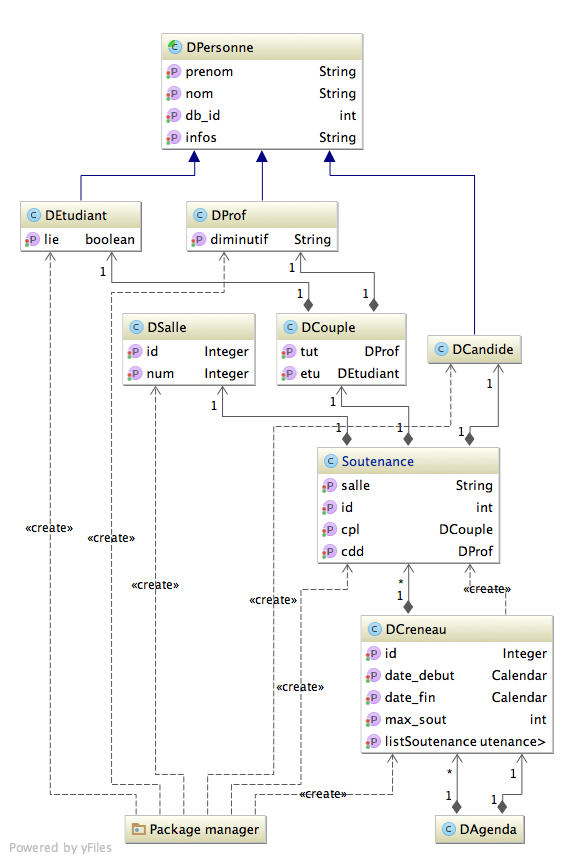
\includegraphics[scale=.5]{uml_don.png}	
				\centering
			\end{figure}

			\paragraph*{}
			Dans ce schéma voit bien l’enchaînement des objets. On commence par les personne et on fini par les agendas. On remarque également que le paquet \textit{manager} crée la totalité objets. Cela vient du fait que les classes de manager instancie ces objets à partir de la base de donnée.

		\subsection{UML de la vue}

			\begin{figure}[h!]
				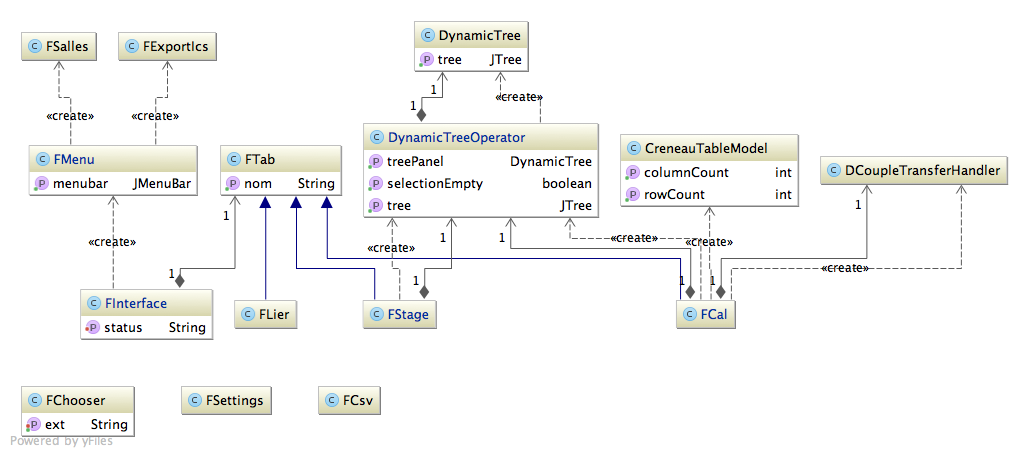
\includegraphics[scale=.5]{uml_fen.png}
				\centering
			\end{figure}

			\paragraph*{}
			Dans ce graphe, on remarque bien que la fenêtre principale (\textit{FInterface}) es composé de d’onglets (\textit{FTab}). On remarque également trois objet hérité de \textit{FTab}, ces dernier constitue les trois onglets de l'application.

	\section{Base de donnée}

		La base de donné est a été conçue à partir du shema UML du modèle montré précédemment. Elle concerne que les données en non la vue ou le contrôleur.

\chapter*{Conclusion}

En espérant avoir été assez claire sur la modélisation de l'application et sur les grande ligne. Nous éspereons que l'application sera repris par un future groupe de projet tuteuré.

\end{document}